\chapter{Depth-first search and Breadth-first search}

\section{Depth-first search (DFS)}

\subsection{Basic DFS implementation}

Write a Depth-first search (DFS) implementation using Sage Graph representation
\begin{itemize}
  \item Write a recursive implementation of the depth-first search.
  \item Add computation of discovery and finishing times to the implementation.
\end{itemize}
(See Handouts on Course Homepage for pseudocode)

\medskip
\begin{sageCell}
def DFS_recursive(G, r):
    """
    Perform DFS from root r. Result is a dictionary mapping a vertex v to
    its predecessor in DFS tree (root is mapped to None).
    """
    prev = {}
    prev[r] = None
    DFS_recursive_call(G, r, prev)
    return prev

def DFS_recursive_call(G, v, prev):
    for u in G.neighbors(v):
        if u not in prev:
            prev[u] = v
            DFS_recursive_call(G, u, prev)
\end{sageCell}

\subsubsection*{Examples}

\begin{sageCell}
   G = Graph({0:[1,2,3], 4:[0,2], 6:[1,2,3,4,5]})

   dfs_dict = DFS_recursive(G, 0)
   dfs_dict
\end{sageCell}
\begin{outCell}
   {0: None, 1: 0, 6: 1, 2: 6, 4: 2, 3: 6, 5: 6}
\end{outCell}

\begin{sageCell}
   G.plot(edge_colors={'red': [(u, v) for (u, v) in dfs_dict.items() if v != None]})
\end{sageCell}
\begin{outImage}
   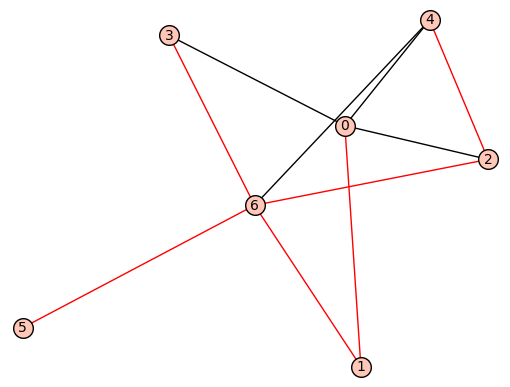
\includegraphics[width=0.5\textwidth]{Images/DFS/dfs_tree.png}
\end{outImage}

\begin{sageCell}
   H = graphs.Grid2dGraph(3, 3)
   DFS_recursive(H, (0, 0))
\end{sageCell}
\begin{outCell}
   {(0, 0): None,
    (0, 1): (0, 0),
    (0, 2): (0, 1),
    (1, 2): (0, 2),
    (1, 1): (1, 2),
    (1, 0): (1, 1),
    (2, 0): (1, 0),
    (2, 1): (2, 0),
    (2, 2): (2, 1)}
\end{outCell}

\subsection{DFS with start (discovery) time and end (finishing) time}

\begin{sageCell}
def DFS_with_times(G, r):
    """
    Perform DFS from root r. Result is a triple of three dictionaries:
    - dictionary mapping a vertex v to its predecessor in DFS tree
      (root is mapped to None).
    - dictionary mapping a vertex to its start time
    - dictionary mapping a vertex to its end time
    """
    global time
    time = 0
    prev = {}
    start = {}
    end = {}
    prev[r] = None
    DFS_with_times_call(G, r, prev, start, end)
    return (prev, start, end)

def DFS_with_times_call(G, v, prev, start, end):
    global time
    time += 1;
    start[v] = time;
    for u in G.neighbors(v):
        if u not in prev:
            prev[u] = v
            DFS_with_times_call(G, u, prev, start, end)
    time += 1;
    end[v] = time;
\end{sageCell}

\subsubsection*{Examples}

\begin{sageCell}
   G = Graph({0:[1,2,3], 4:[0,2], 6:[1,2,3,4,5]})
   (prev, disc, finish) = DFS_with_times(G, 0)
   (prev, disc, finish)
\end{sageCell}
\begin{outCell}
   ({0: None, 1: 0, 2: 6, 3: 6, 4: 2, 5: 6, 6: 1},
    {0: 1, 1: 2, 2: 4, 3: 8, 4: 5, 5: 10, 6: 3},
    {0: 14, 1: 13, 2: 7, 3: 9, 4: 6, 5: 11, 6: 12})
\end{outCell}

\begin{sageCell}
    G.relabel(dict([(v, (disc[v], finish[v])) for v in G.vertices()]))
    G.plot(edge_colors={'red': [((disc[u],finish[u]), (disc[v],finish[v]))
      for (u, v) in prev.items() if v != None]})
\end{sageCell}
\begin{outImage}
   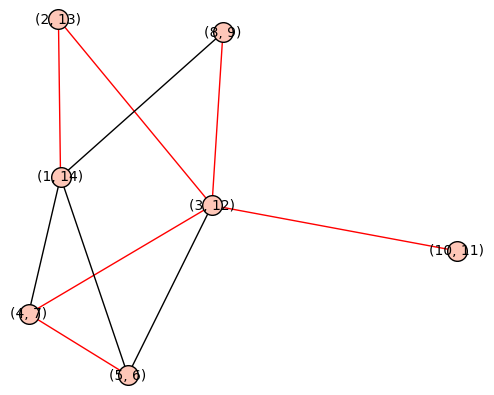
\includegraphics[width=0.6\textwidth]{Images/DFS/dfs_tree_with_times.png}
\end{outImage}

\section{Breadth-first search (BFS)}

Write a Breadth-first search (BFS) implementation using Sage Graph representation.

\medskip
\begin{sageCell}
import queue
def BFS(G, r):
    """
    Perform BFS from root r. Result is a dictionary mapping a vertex v
    to its predecessor in BFS tree (root is mapped to None).
    """
    prev = {}
    prev[r] = None
    q = queue.Queue()
    q.put(r)
    while not q.empty():
        v = q.get()
        for u in G.neighbors(v):
            if u not in prev:
                prev[u] = v
                q.put(u)
    return prev
\end{sageCell}

\subsubsection*{Example}

\begin{sageCell}
    BFS(H, (0, 0))
\end{sageCell}
\begin{outCell}
   {(0, 0): None,
    (0, 1): (0, 0),
    (1, 0): (0, 0),
    (0, 2): (0, 1),
    (1, 1): (0, 1),
    (2, 0): (1, 0),
    (1, 2): (0, 2),
    (2, 1): (1, 1),
    (2, 2): (1, 2)}
\end{outCell}

\section{Topological sorting}

\begin{itemize}
\item Use DFS with discovery and finishing times to implement topological sorting of a DAG (directed acyclic) graph
\item Help professor Bumstead to dress himself in the correct order. Order of putting his garments is given by the digraph below
\end{itemize}

\begin{sageCell}
    T = DiGraph({'undershorts': ['shoes','pants'],'pants':['shoes','belt'],'belt':['jacket'],'shirt':['belt','tie'],'tie':['jacket'],'socks':['shoes'],'watch':[]})
\end{sageCell}

\begin{sageCell}
def DFS_DiGraph(G):
    """
    Implement (recursive) DFS on a digraph to create a
    "forest of DFS trees"

    Use G.neighbors_out(v) to get "out" neighbors of vertex v
    """
    global time
    time = 0
    prev = {}
    start = {}
    end = {}
    for v in G.vertices(sort=False):
        if v not in prev:
            prev[v] = None
            DFS_DiGraph_call(G, v, prev, start, end)
    return (prev, start, end)

def DFS_DiGraph_call(G, v, prev, start, end):
    global time
    time += 1;
    start[v] = time;
    for u in G.neighbor_out_iterator(v):
        if u not in prev:
            prev[u] = v
            DFS_DiGraph_call(G, u, prev, start, end)
    time += 1
    end[v] = time
\end{sageCell}

\begin{sageCell}
    DFS_DiGraph(T)
\end{sageCell}
\begin{outCell}
    ({'belt': None,
      'jacket': 'belt',
      'tie': None,
      'watch': None,
      'shoes': None,
      'socks': None,
      'pants': None,
      'undershorts': None,
      'shirt': None},
     {'belt': 1,
      'jacket': 2,
      'tie': 5,
      'watch': 7,
      'shoes': 9,
      'socks': 11,
      'pants': 13,
      'undershorts': 15,
      'shirt': 17},
     {'jacket': 3,
      'belt': 4,
      'tie': 6,
      'watch': 8,
      'shoes': 10,
      'socks': 12,
      'pants': 14,
      'undershorts': 16,
      'shirt': 18})
\end{outCell}

\begin{sageCell}
def topological_sort(G):
    """
    Performs topological sort on a DAG (directed acyclic graph) G
    (calculate finishing times and sort vertices by them in
    descending order)
    """
    (_, _, finish) = DFS_DiGraph(T)
    return sorted(finish.items(), key=lambda x: -x[1])
\end{sageCell}

\begin{sageCell}
    topological_sort(T)
\end{sageCell}
\begin{outCell}
    [('shirt', 18),
     ('undershorts', 16),
     ('pants', 14),
     ('socks', 12),
     ('shoes', 10),
     ('watch', 8),
     ('tie', 6),
     ('belt', 4),
     ('jacket', 3)]
\end{outCell}
